% !TeX root = Thesis.tex

\chapter{Experiments~and~Results}
\label{chap:experiments_and_results}

We conduct experiments to gauge the performance of different configurations for CSG-CRN and explore its capabilities.\footnote{\raggedright All datasets and trained model used in the experiments are available at: \href{https://huggingface.co/datasets/AlexWolski/CSGCRN-SDF-Dataset}{\nolinkurl{huggingface.co/datasets/AlexWolski/CSGCRN-SDF-Dataset}}}

\section{Reconstruction~Loss~Metric~Comparison}
\label{sec:reconstruction_loss_comparison}

The CSG-CRN architecture implements a unique combination of SDF volumes, constructive solid geometry, and cascaded refinement. A fine-tuned loss function is required to compensate for the complications presented by the architecture and stabilize training. Auxiliary loss metrics are used to help control the results, but the the reconstruction loss metric ultimately determines the quality of the model.

We experiment with six reconstruction loss metrics: Chamfer Distance (CD), L1, Logarithmic (LOG), Mean Squared Error (MSE), Occupancy (OCC), and Sigmoid (SIG).  All training runs were performed with Separate model parameters, 9 primitives (3 per cascade x 3 cascades), and 2048 input and loss samples. The model was trained on the Airplane category of the ShapeNet dataset with 3237 training, 404 validation, and 404 testing samples. All training was performed on an RTX 3080 graphics card. The scheduler was configured to lower the learning rate after 20 epochs without improvement and stop training a cascade after 40 cascades without improvement. All testing was performed with 10000 samples and a Marching Cubes resolution of 512.

The sigmoid loss performed best in the CD and EMD testing metrics while LOG loss performed best in IoU. Although the sigmoid model wins in two metrics, a visual inspection reveals that the reconstruction is missing tail fins, the nose, and has warped wings. In contrast, the LOG loss airplane output is smoother and has more complete wings. All subsequent experiments are conducted with LOG loss and an emphasis on the IoU metric.



\begin{figure}[ht]
	\centering
	\begin{subfigure}{0.13\textwidth}
		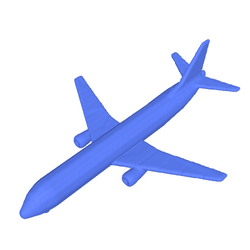
\includegraphics[width=\linewidth]{Images/Loss Function Renders/TARGET.png}
		\caption{Target}
	\end{subfigure}
	\hfill
	\begin{subfigure}{0.13\textwidth}
		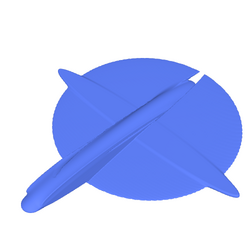
\includegraphics[width=\linewidth]{Images/Loss Function Renders/CHAMFER.png}
		\caption{CD}
	\end{subfigure}
	\hfill
	\begin{subfigure}{0.13\textwidth}
		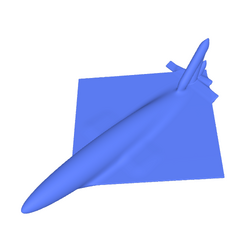
\includegraphics[width=\linewidth]{Images/Loss Function Renders/L1.png}
		\caption{L1}
	\end{subfigure}
	\hfill
	\begin{subfigure}{0.13\textwidth}
		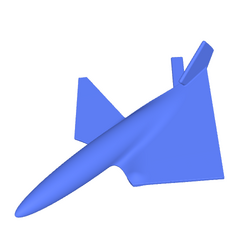
\includegraphics[width=\linewidth]{Images/Loss Function Renders/LOG.png}
		\caption{LOG}
	\end{subfigure}
	\hfill
	\begin{subfigure}{0.13\textwidth}
		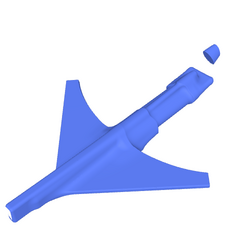
\includegraphics[width=\linewidth]{Images/Loss Function Renders/MSE.png}
		\caption{MSE}
	\end{subfigure}
	\hfill
	\begin{subfigure}{0.13\textwidth}
		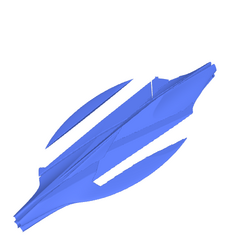
\includegraphics[width=\linewidth]{Images/Loss Function Renders/OCC.png}
		\caption{OCC}
	\end{subfigure}
	\hfill
	\begin{subfigure}{0.13\textwidth}
		
\includegraphics[width=\linewidth]{Images/Loss Function Renders/SIG.png}
		\caption{SIG}
	\end{subfigure}
	\caption{Comparison of output shapes across six different reconstruction loss metrics.}
	\label{fig:loss_function_renders}
\end{figure}

\begin{table}[ht]
	\centering
	\label{tab:loss_function_comparison}
	\singlespace
	\footnotesize
	\setlength{\tabcolsep}{3pt}
	\setcellgapes{4pt}
	\makegapedcells
	% Fake a semi-bold font that doesn't resize text.
	\renewcommand{\bfdefault}{b}
	\begin{tabular}{|l|r|r|r|r|r|r|r|r|r|}
		\hline
		\makecell{Loss\\Function} & \makecell{Best\\Loss} & \makecell{Best\\CD} & \makecell{Best\\EMD} & \makecell{Best\\IoU} & \makecell{Batch\\Size} & \makecell{Peak GPU\\(GB)} & \makecell{Train Time\\(min)} & \makecell{Best\\Epoch} & \makecell{Total\\Epochs} \\
		\Xhline{1pt}
		CD  & 155.8787 & 155.78         & 1488.4         & 0.3002          & 5  & 9.4 & 1441.4 & 180 & 203 \\
		L1  & 0.0303   & 77.81          & 1012.1         & 0.4415          & 72 & 7.2 & 50.9   & 294 & 310 \\
		LOG & 0.2981   & 81.23          & 1010.1         & \textbf{0.4750} & 72 & 7.2 & 51.9   & 294 & 301 \\
		MSE & 0.0027   & 71.97          & 938.5          & 0.3714          & 72 & 7.2 & 36.7   & 200 & 206 \\
		OCC & 0.5527   & 221.47         & 1345.5         & 0.2536          & 72 & 6.2 & 33.9   & 182 & 216 \\
		SIG & 0.2910   & \textbf{61.44} & \textbf{786.5} & 0.3992          & 72 & 6.6 & 55.3   & 270 & 310 \\
		\hline
	\end{tabular}
	\caption{Performance comparison of six different reconstruction loss metrics. Lower is better for CD and EMD. Higher is better for IoU.}
\end{table}


\section{Surface-Uniform~Ratio}
\label{sec:surface_uniform_ratio_experiment}

We experiment with different ratios of near-surface samples to uniformly distributed samples used for the model input and loss computation. Models were trained on Surface-Uniform ratios ranging from 0.0 (only near surface) to 1.0 (only uniform). We test two loss functions with the best visual accuracy from the previous experiment: L1 and LOG. A new model was trained for each combination of loss function and Surface-Uniform ratio value. Each configuration was trained three times on separate seeds to get an average result, totaling 66 trained models. The same configuration as the \nameref{sec:reconstruction_loss_comparison} experiment was used, except for the input samples being reduced to 1024.

The trend lines for the CD and EMD metrics are inconclusive due to high variance. But the IoU metric shows a statistically significant result with $p < 0.001$ for both loss functions. The results indicate that a Surface-Uniform ratio of 0.0 produces marginally better results, so we used this configuration for all subsequent experiments.


\begin{figure}[ht]
	\centering
	\begin{subfigure}{0.32\textwidth}
		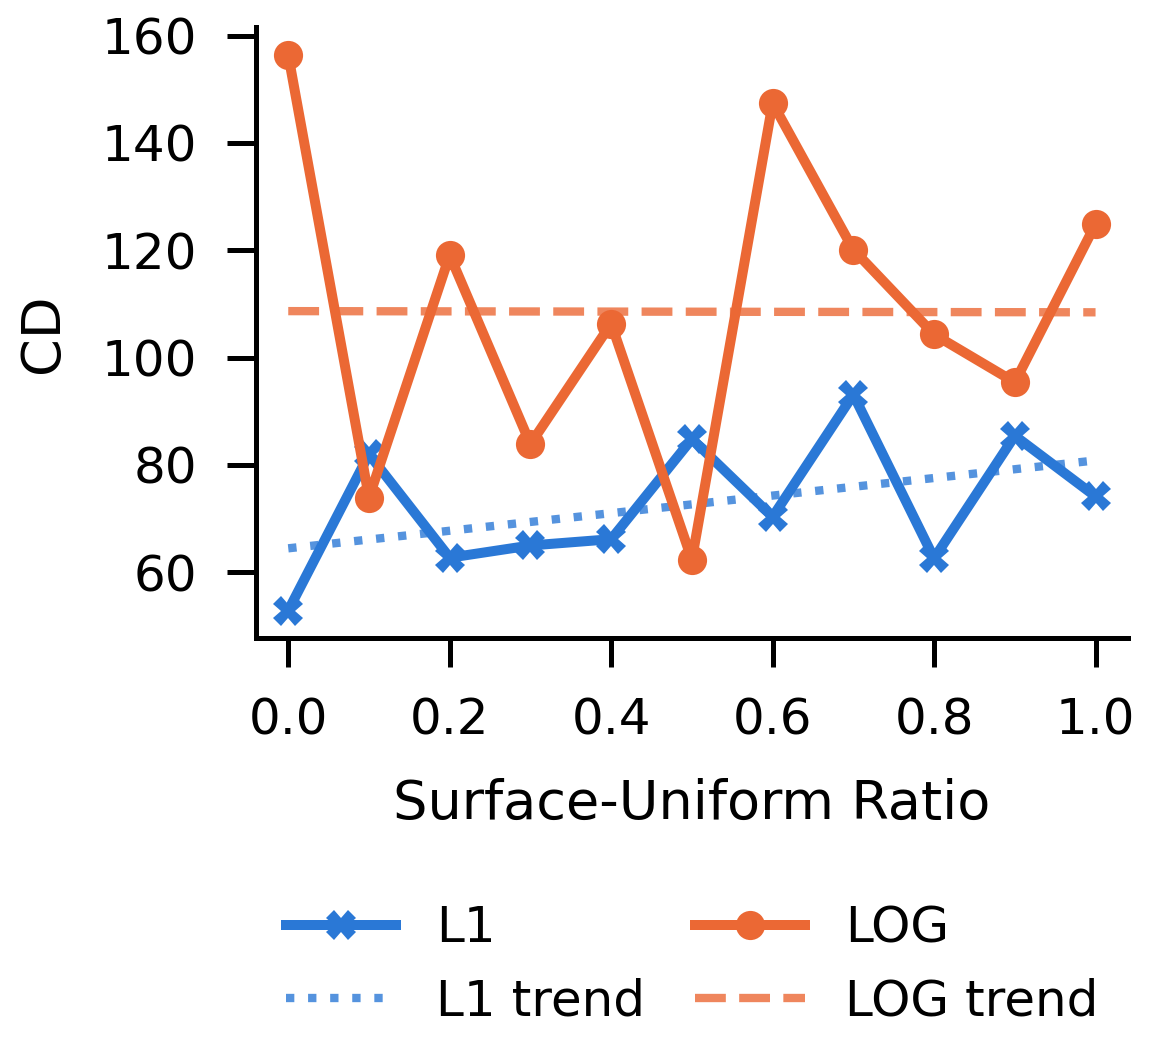
\includegraphics[width=\linewidth]{Images/Surface Uniform Ratio Figures/Surface Uniform Ratio Chamfer.png}
		\caption{CD vs Surface-Uniform Ratio. Lower is better.}
	\end{subfigure}
	\hfill
	\begin{subfigure}{0.32\textwidth}
		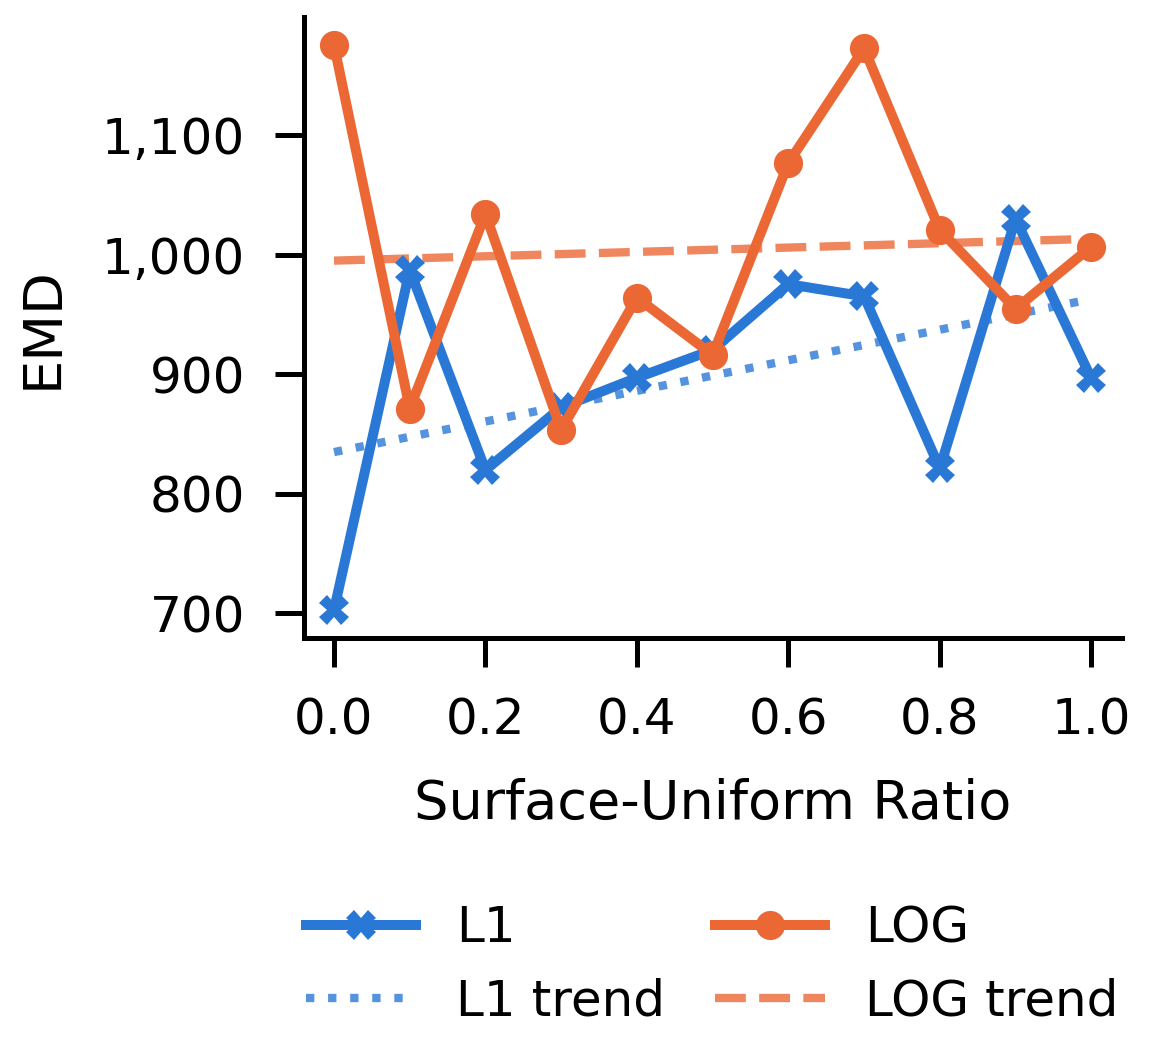
\includegraphics[width=\linewidth]{Images/Surface Uniform Ratio Figures/Surface Uniform Ratio EMD.png}
		\caption{EMD vs Surface-Uniform Ratio. Lower is better.}
	\end{subfigure}
	\hfill
	\begin{subfigure}{0.32\textwidth}
		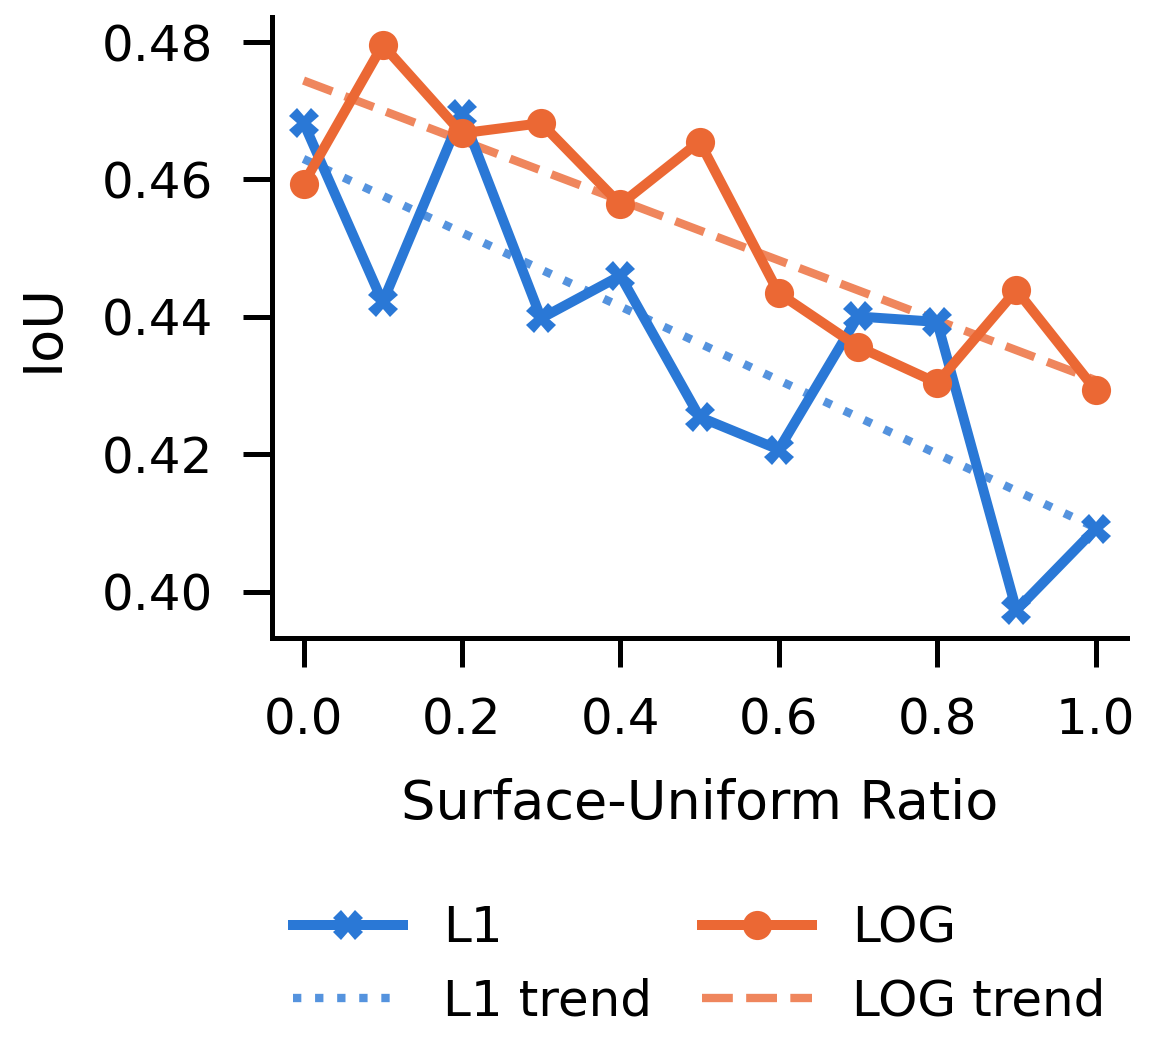
\includegraphics[width=\linewidth]{Images/Surface Uniform Ratio Figures/Surface Uniform Ratio IoU.png}
		\caption{IoU vs Surface-Uniform Ratio. Higher is better.}
	\end{subfigure}
	\caption{}
	\label{fig:surface_uniform_ratio}
\end{figure}


\section{Input~Sample~Size}
\label{sec:input_size_experiment}

The encoder network size is correlated with performance and training time. A benchmark test is conducted to determine the configuration that produces the best reconstructions. The number of SDF point sample inputs is increased together with the number of sample points used for loss computation. The same model configuration was used as the \nameref{sec:reconstruction_loss_comparison} experiment except we use the LOG metric for all runs. We double the model size for each test starting with 128 and ending at 16384. Each training run was limited to 3.5 GiB of GPU memory with the batch size maximized for the available memory. Holding GPU memory constant for all runs allows for comparing training times and measuring the performance degradation from oversize models.

Predictably, the training time trends upward as we increase the encoder size. The variance in training time is caused by the early-stop mechanism ending some runs short. The 512 input size model was only 54\% slower than the 128 input size run despite having a 4x larger encoder and training for the same number of epochs. This is because the decoder network comprises the majority of the model at these small input sizes. In contrast, the 16384 input size model is 76\% larger than the 16384 input size model.

The 512 input size model has the best results in CD and EMD while the 8192 input size model had the best result in IoU. The 512 input size model has qualitatively worse reconstructions than the larger models, further showing the CD and EMD metrics are not good measures of visual quality. The 16384 input size model produces warped outputs and ranks only fourth best in IoU score despite being the largest. This is due to the low batch size.

\begin{figure}[ht]
	\centering
	\begin{subfigure}{0.13\textwidth}
		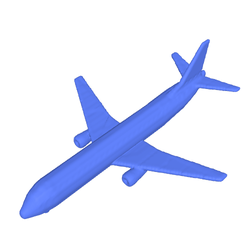
\includegraphics[width=\linewidth]{Images/Input Size Renders/TARGET.png}
		\caption{Target}
	\end{subfigure}

	\begin{subfigure}{0.13\textwidth}
		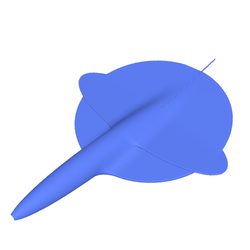
\includegraphics[width=\linewidth]{Images/Input Size Renders/128.png}
		\caption{128}
	\end{subfigure}
	\hspace{0.03\textwidth}
	\begin{subfigure}{0.13\textwidth}
		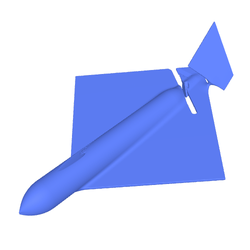
\includegraphics[width=\linewidth]{Images/Input Size Renders/256.png}
		\caption{256}
	\end{subfigure}
	\hspace{0.03\textwidth}
	\begin{subfigure}{0.13\textwidth}
		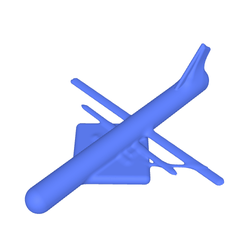
\includegraphics[width=\linewidth]{Images/Input Size Renders/512.png}
		\caption{512}
	\end{subfigure}
	\hspace{0.03\textwidth}
	\begin{subfigure}{0.13\textwidth}
		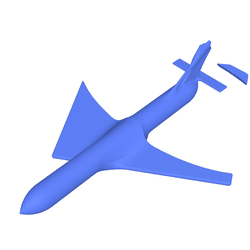
\includegraphics[width=\linewidth]{Images/Input Size Renders/1024.png}
		\caption{1024}
	\end{subfigure}

	\begin{subfigure}{0.13\textwidth}
		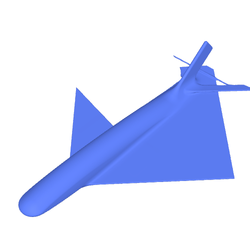
\includegraphics[width=\linewidth]{Images/Input Size Renders/2048.png}
		\caption{2048}
	\end{subfigure}
	\hspace{0.03\textwidth}
	\begin{subfigure}{0.13\textwidth}
		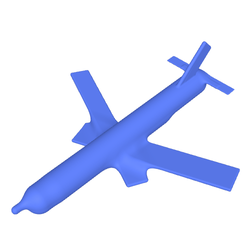
\includegraphics[width=\linewidth]{Images/Input Size Renders/4096.png}
		\caption{4096}
	\end{subfigure}
	\hspace{0.03\textwidth}
	\begin{subfigure}{0.13\textwidth}
		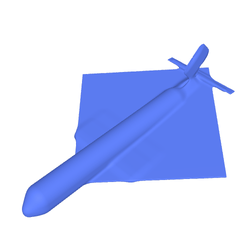
\includegraphics[width=\linewidth]{Images/Input Size Renders/8192.png}
		\caption{8192}
	\end{subfigure}
	\hspace{0.03\textwidth}
	\begin{subfigure}{0.13\textwidth}
		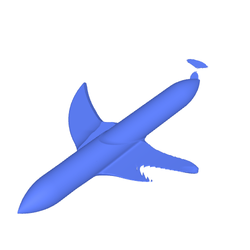
\includegraphics[width=\linewidth]{Images/Input Size Renders/16384.png}
		\caption{16384}
	\end{subfigure}
	\caption{Comparison of output shapes across models trained on eight different input and loss sample sizes.}
	\label{fig:input_size_renders}
\end{figure}

\begin{table}[ht]
	\centering
	\singlespace
	\footnotesize
	\setlength{\tabcolsep}{3pt}
	\setcellgapes{4pt}
	\makegapedcells
	\renewcommand{\bfdefault}{b}
	\begin{tabular}{|r|r|r|r|r|r|r|r|r|}
		\hline
		\makecell{Input/Loss\\Samples} & \makecell{Best\\Loss} & \makecell{Best\\CD} & \makecell{Best\\EMD} & \makecell{Best\\IoU} & \makecell{Batch\\Size} & \makecell{Train Time\\(min)} & \makecell{Best\\Epoch} & \makecell{Total\\Epochs} \\
		\Xhline{1pt}
		128   & 0.3205 & 247.62         & 1440.1         & 0.3876          & 404 & 17.0  & 270 & 292 \\
		256   & 0.3135 & 341.19         & 1769.8         & 0.4286          & 327 & 14.2  & 234 & 236 \\
		512   & 0.3020 & \textbf{71.87} & \textbf{741.6} & 0.4614          & 160 & 26.1  & 283 & 291 \\
		1024  & 0.2942 & 82.79          & 837.0          & 0.4871          & 81  & 27.0  & 192 & 206 \\
		2048  & 0.2904 & 97.69          & 1113.7         & 0.4808          & 40  & 69.0  & 309 & 313 \\
		4096  & 0.3075 & 82.17          & 959.1          & 0.4678          & 20  & 80.1  & 154 & 185 \\
		8192  & 0.2682 & 161.90         & 1252.3         & \textbf{0.5272} & 10  & 183.2 & 243 & 257 \\
		16384 & 0.3091 & 184.87         & 1043.3         & 0.4759          & 5   & 322.1 & 198 & 238 \\
		\hline
	\end{tabular}
	\caption{Performance and training time comparison of eight input and loss sample size configurations. Lower is better for CD and EMD. Higher is better for IoU.}
	\label{tab:input_size_comparison}
\end{table}


\section{Cascaded~Refinement~Configuration~and~Training~Mode}
\label{sec:prims_per_cascade_experiment}

This section compares the cascaded refinement architecture against the end-to-end architecture of all previous work in primitive 3D reconstruction. All experiments are normalized to use a maximum of 10 GiB of video RAM and output 16 output primitives. One CSG-CRN model is trained to predict 16 primitives in one pass to serve as the end-to-end model baseline. And eight CSG-CRN models are trained to compare the cascaded refinement configurations. The four cascade configurations resulting in 16 primitives are eight, four, two, and one primitives per pass with two, four, eight, and sixteen passes respectively. We train models with both separate and shared parameters for a total of 8 trained cascading models.

The results show that the shared parameter models overall outperform the separate parameters across the board. All shared models have a lower IoU than the corresponding separate model except for the 2 primitive $\times$ 8 passes configuration outlier. The 8 primitive $\times$ 2 pass shared parameter model ranks best in all metrics by a large margin, including the single-pass baseline. The 4 primitive $\times$ 4 passes shared model also outperforms the baseline, but none of the shared parameter models do. For both shared and separate parameter models, the performance trends downward as the number of cascades increases. The primary cause is an increase in greedy primitive fitting behavior where the initial cascade struggles to represent the entire target with a limited number of primitives. Then each subsequent cascade works off of a bad foundation.

An additional result of interest is the total network size. All separate parameter models are larger than the baseline single-pass model since the network weights are duplicated for each cascade. In contrast, all shared parameter models are smaller than the baseline since the same network weights are running inference multiple times. The 4 primitive $\times$ 4 pass shared model performed better than baseline at less than 30\% of the network size. Despite the smaller size, the shared model took 20\% longer to train since it trains on both the initial pass and the refinement pass.


\begin{figure}[ht]
	\centering
	\captionsetup[subfigure]{justification=centering}
	\begin{subfigure}[t]{0.17\textwidth}
		\centering
		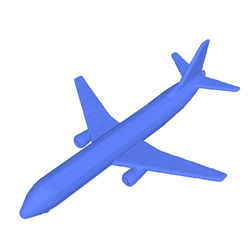
\includegraphics[width=0.765\linewidth]{Images/Cascade Output Size Renders/TARGET.png}
		\caption{Target}
	\end{subfigure}
	\hspace{0.01\textwidth}
	\begin{subfigure}[t]{0.17\textwidth}
		\centering
		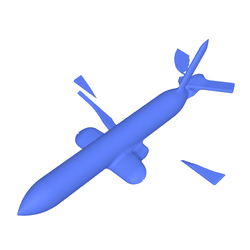
\includegraphics[width=0.765\linewidth]{Images/Cascade Output Size Renders/Single Pass 16x1.png}
		\caption{Single Pass 16x1}
	\end{subfigure}

	\begin{subfigure}[t]{0.17\textwidth}
		\centering
		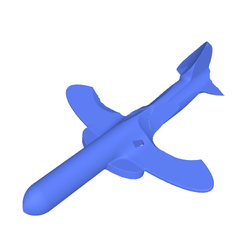
\includegraphics[width=0.765\linewidth]{Images/Cascade Output Size Renders/Separate 8x2.png}
		\caption{Separate 8x2}
	\end{subfigure}
	\hspace{0.01\textwidth}
	\begin{subfigure}[t]{0.17\textwidth}
		\centering
		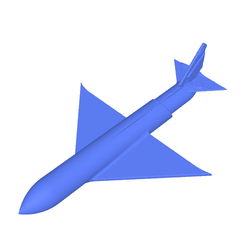
\includegraphics[width=0.765\linewidth]{Images/Cascade Output Size Renders/Separate 4x4.png}
		\caption{Separate 4x4}
	\end{subfigure}
	\hspace{0.01\textwidth}
	\begin{subfigure}[t]{0.17\textwidth}
		\centering
		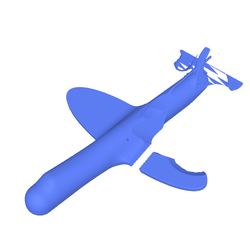
\includegraphics[width=0.765\linewidth]{Images/Cascade Output Size Renders/Separate 2x8.png}
		\caption{Separate 2x8}
	\end{subfigure}
	\hspace{0.01\textwidth}
	\begin{subfigure}[t]{0.17\textwidth}
		\centering
		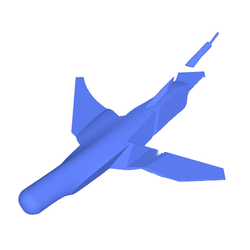
\includegraphics[width=0.765\linewidth]{Images/Cascade Output Size Renders/Separate 1x16.png}
		\caption{Separate 1x16}
	\end{subfigure}

	\begin{subfigure}[t]{0.17\textwidth}
		\centering
		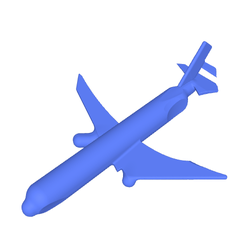
\includegraphics[width=0.765\linewidth]{Images/Cascade Output Size Renders/Shared 8x2.png}
		\caption{Shared 8x2}
	\end{subfigure}
	\hspace{0.01\textwidth}
	\begin{subfigure}[t]{0.17\textwidth}
		\centering
		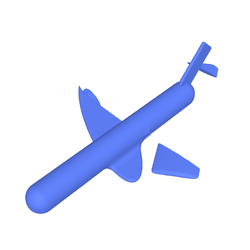
\includegraphics[width=0.765\linewidth]{Images/Cascade Output Size Renders/Shared 4x4.png}
		\caption{Shared 4x4}
	\end{subfigure}
	\hspace{0.01\textwidth}
	\begin{subfigure}[t]{0.17\textwidth}
		\centering
		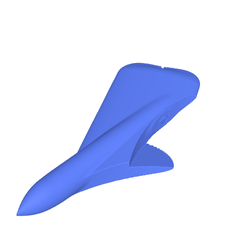
\includegraphics[width=0.765\linewidth]{Images/Cascade Output Size Renders/Shared 2x8.png}
		\caption{Shared 2x8}
	\end{subfigure}
	\hspace{0.01\textwidth}
	\begin{subfigure}[t]{0.17\textwidth}
		\centering
		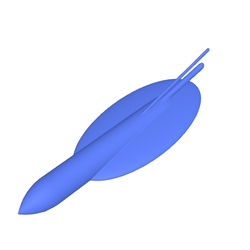
\includegraphics[width=0.765\linewidth]{Images/Cascade Output Size Renders/Shared 1x16.png}
		\caption{Shared 1x16}
	\end{subfigure}
	\caption{Comparison of output shapes across models trained on different cascaded refinement configurations. A single pass model (top right) serves as a baseline. The configuration format is $primitives\;per\;cascade \times number\;of\;cascades$.}
	\label{fig:prims_per_cascade_renders}
\end{figure}

\begin{table}[ht]
	\centering
	\singlespace
	\footnotesize
	\setlength{\tabcolsep}{3pt}
	\setcellgapes{4pt}
	\makegapedcells
	\renewcommand{\bfdefault}{b}
	\begin{tabular}{|l|r|r|r|r|r|r|r|r|r|r|}
		\hline
		\makecell{Training\\Mode} & \makecell{Prims x\\Cascades} & \makecell{Best\\Loss} & \makecell{Best\\CD} & \makecell{Best\\EMD} & \makecell{Best\\IoU} & \makecell{Batch\\Size} & \makecell{Params\\(M)} & \makecell{Train Time\\(min)} & \makecell{Best\\Epoch} & \makecell{Total\\Epochs} \\
		\Xhline{1pt}
		\makecell[l]{Single\\Pass} & 16x1 & 0.2714 & 73.68          & 574.8          & 0.5315          & 122 & 69.9  & 35.1  & 110  & 150  \\
		\hline
		\multirow{4}{*}{Separate} & 8x2  & 0.2844 & 43.36          & 641.6          & 0.5103          & 170 & 72.7  & 39.1  & 245  & 256  \\
		                          & 4x4  & 0.2791 & 62.80          & 632.9          & 0.5282          & 207 & 78.4  & 39.1  & 327  & 332  \\
		                          & 2x8  & 0.2902 & 109.83         & 880.3          & 0.5055          & 230 & 89.6  & 66.6  & 541  & 581  \\
		                          & 1x16 & 0.3252 & 140.88         & 875.6          & 0.4277          & 234 & 112.1 & 122.6 & 1115 & 1147 \\
		\hline
		\multirow{4}{*}{Shared}   & 8x2  & 0.2301 & \textbf{14.36} & \textbf{489.3} & \textbf{0.6054} & 181 & 36.3  & 43.5  & 147  & 187  \\
		                          & 4x4  & 0.2627 & 34.91          & 522.1          & 0.5586          & 375 & 19.6  & 42.3  & 133  & 173  \\
		                          & 2x8  & 0.3344 & 184.61         & 1225.9         & 0.3963          & 404 & 11.2  & 64.1  & 144  & 160  \\
		                          & 1x16 & 0.3407 & 222.42         & 924.2          & 0.4334          & 404 & 7.0   & 183.5 & 254  & 269  \\
		\hline
	\end{tabular}
	\caption{Performance, network size, and training time comparison of eight cascaded refinement configurations. Lower is better for CD and EMD. Higher is better for IoU.}
	\label{tab:prims_per_cascade_comparison}
\end{table}


\section{ShapeNet~Benchmark}
\label{sec:shapenet_experiment}

We apply the most effective training configuration found in the previous experiment to train on the ShapeNet dataset. Five models are trained separately on curated shape categories airplane, bench, car, char, and sofa. In addition, one model is trained on all 54 shape categories in ShapeNet. All models are trained with a data split of 80\% training, 10\% validation, and 10\% testing. For the model trained on all samples, this translates to 41367 test samples and 5137 samples each for validation and testing. We choose 1024 input samples and 2048 loss samples to reduce model complexity and size. The chosen loss sample size is larger since it provides higher accuracy without affecting the size of the model. Each model outputs 16 primitives per pass for 3 passes totaling 48 primitives. Unlike previous experiments, we limit the model to 4 subtract operations per pass to encourage prediction of smaller details. Each model is trained with a batch size of 64. All other configurations are identical to previous experiments.

Both the models trained on one shape category and the model trained on the entire dataset show strong results. The Sofa category has the highest overall accuracy with an average IoU over 0.8. The Bench category has the lowest average IoU at around 0.52, since the point cloud input struggles to encode benches with thin slats and gaps at a 1024 input sample resolution. The models trained on a single shape category perform significantly better on all categories except for Benches where the results are roughly even.

A visual inspection reveals that the models trained on single shape categories have better blending and continuity. This is especially apparent in the car reconstructions where the primitives are blended to the point they can not be distinguished as separate shapes. The whole-dataset model has good volumetric accuracy but misses smaller details. The generalized model produces results with holes, gaps, and lumpy surfaces.

\newpage


\begin{figure}[ht]
	\centering
	\captionsetup[subfigure]{justification=centering}
	\begin{subfigure}{\textwidth}
		\centering
		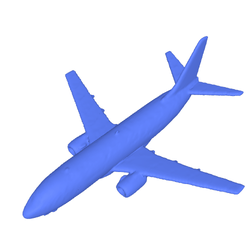
\includegraphics[width=0.13\textwidth]{Images/ShapeNet Benchmark Renders/Airplane TARGET.png}
		\hspace{0.03\textwidth}
		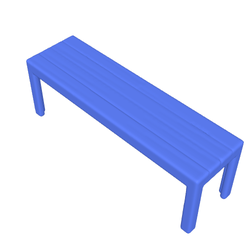
\includegraphics[width=0.13\textwidth]{Images/ShapeNet Benchmark Renders/Bench TARGET.png}
		\hspace{0.03\textwidth}
		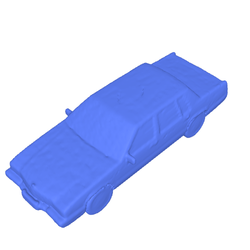
\includegraphics[width=0.13\textwidth]{Images/ShapeNet Benchmark Renders/Car TARGET.png}
		\hspace{0.03\textwidth}
		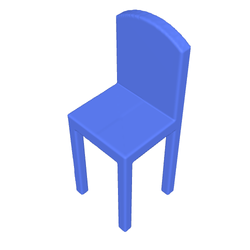
\includegraphics[width=0.13\textwidth]{Images/ShapeNet Benchmark Renders/Chair TARGET.png}
		\hspace{0.03\textwidth}
		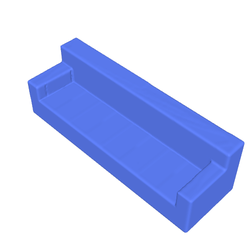
\includegraphics[width=0.13\textwidth]{Images/ShapeNet Benchmark Renders/Sofa TARGET.png}
		\caption{Target}
	\end{subfigure}

	\begin{subfigure}{\textwidth}
		\centering
		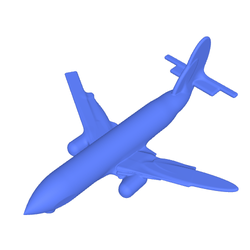
\includegraphics[width=0.13\textwidth]{Images/ShapeNet Benchmark Renders/Airplane Single Category.png}
		\hspace{0.03\textwidth}
		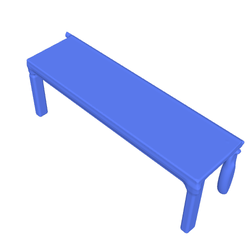
\includegraphics[width=0.13\textwidth]{Images/ShapeNet Benchmark Renders/Bench Single Category.png}
		\hspace{0.03\textwidth}
		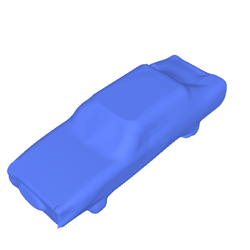
\includegraphics[width=0.13\textwidth]{Images/ShapeNet Benchmark Renders/Car Single Category.png}
		\hspace{0.03\textwidth}
		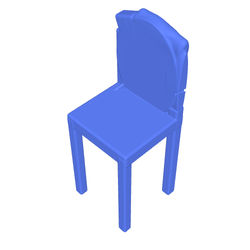
\includegraphics[width=0.13\textwidth]{Images/ShapeNet Benchmark Renders/Chair Single Category.png}
		\hspace{0.03\textwidth}
		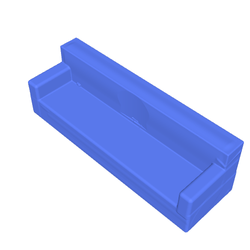
\includegraphics[width=0.13\textwidth]{Images/ShapeNet Benchmark Renders/Sofa Single Category.png}
		\caption{Single-Category Training}
	\end{subfigure}

	\begin{subfigure}{\textwidth}
		\centering
		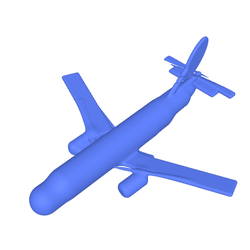
\includegraphics[width=0.13\textwidth]{Images/ShapeNet Benchmark Renders/Airplane Whole Dataset.png}
		\hspace{0.03\textwidth}
		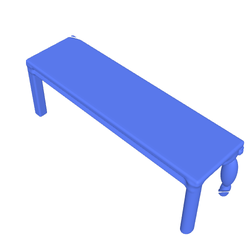
\includegraphics[width=0.13\textwidth]{Images/ShapeNet Benchmark Renders/Bench Whole Dataset.png}
		\hspace{0.03\textwidth}
		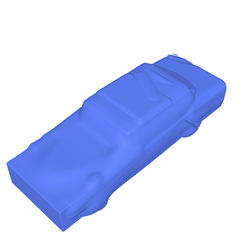
\includegraphics[width=0.13\textwidth]{Images/ShapeNet Benchmark Renders/Car Whole Dataset.png}
		\hspace{0.03\textwidth}
		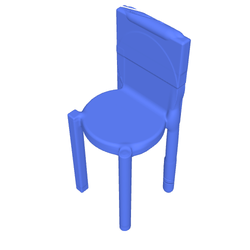
\includegraphics[width=0.13\textwidth]{Images/ShapeNet Benchmark Renders/Chair Whole Dataset.png}
		\hspace{0.03\textwidth}
		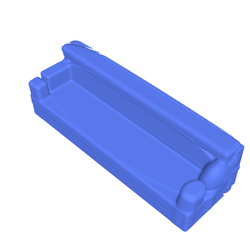
\includegraphics[width=0.13\textwidth]{Images/ShapeNet Benchmark Renders/Sofa Whole Dataset.png}
		\caption{All-Category Training}
	\end{subfigure}
	\caption{Comparison of output shapes for models trained on one shape category (second row) versus trained on the whole of the ShapeNet dataset (third row.)}
	\label{fig:shapenet_benchmark_renders}
\end{figure}

\begin{table}[ht]
	\centering
	\singlespace
	\footnotesize
	\setlength{\tabcolsep}{3pt}
	\setcellgapes{4pt}
	\makegapedcells
	\renewcommand{\bfdefault}{b}
	\begin{tabular}{|l|l|r|r|r|r|r|r|r|r|}
		\hline
		\makecell{Shape\\Category} & \makecell{Training\\Set} & \makecell{Best\\Loss} & \makecell{Best\\CD} & \makecell{Best\\EMD} & \makecell{Best\\IoU} & \makecell{Batch\\Size} & \makecell{Train Time\\(min)} & \makecell{Best\\Epoch} & \makecell{Total\\Epochs} \\
		\Xhline{1pt}
		\multirow{2}{*}{Airplane} & \smash[b]{Single Category} & 0.1999 & \textbf{9.78}  & \textbf{395.6} & \textbf{0.6883} & 64 & 199.7 & 165 & 205 \\
		                          & Whole Dataset              & 0.2218 & 13.29          & 461.9          & 0.6150          & 64 & 685.8 & 42  & 52  \\
		\hline
		\multirow{2}{*}{Bench}    & \smash[b]{Single Category} & 0.2193 & 21.37          & 488.4          & 0.5202          & 64 & 76.3  & 148 & 188 \\
		                          & Whole Dataset              & 0.2156 & \textbf{16.02} & \textbf{473.8} & \textbf{0.5234} & 64 & 685.8 & 42  & 52  \\
		\hline
		\multirow{2}{*}{Car}      & \smash[b]{Single Category} & 0.2295 & \textbf{19.45} & \textbf{481.1} & \textbf{0.6859} & 64 & 181.9 & 157 & 197 \\
		                          & Whole Dataset              & 0.2476 & 23.65          & 565.4          & 0.6646          & 64 & 685.8 & 42  & 52  \\
		\hline
		\multirow{2}{*}{Chair}    & \smash[b]{Single Category} & 0.2176 & \textbf{18.11} & \textbf{471.6} & \textbf{0.6683} & 64 & 283.9 & 163 & 203 \\
		                          & Whole Dataset              & 0.2413 & 25.94          & 578.6          & 0.6076          & 64 & 685.8 & 42  & 52  \\
		\hline
		\multirow{2}{*}{Sofa}     & \smash[b]{Single Category} & 0.2074 & 16.97          & \textbf{438.6} & \textbf{0.8069} & 64 & 138.8 & 159 & 199 \\
		                          & Whole Dataset              & 0.2104 & \textbf{15.83} & 441.2          & 0.8013          & 64 & 685.8 & 42  & 52  \\
		\hline
		\makecell[l]{All}         & Whole Dataset           & 0.2261 & 23.38          & 541.9                     & 0.6440          & 64 & 685.8 & 42  & 52  \\
		\hline
	\end{tabular}
	\caption{Performance and training time comparison the five models trained on a single shape category each against one model trained on all 54 shape categories of the ShapeNet dataset.}
	\label{tab:shapenet_benchmark_comparison}
\end{table}


\section{Unseen~Shape~Class~Reconstruction}
\label{sec:unseen_class_experiment}

The model trained on the ShapeNet dataset can be used to reconstruct unseen shape categories. To demonstrate, we run inference on the Person, Sink, and Stairs categories from the ModelNet40 dataset~\cite{Wu2015}.

The reconstruction quality of the unseen shape categories is much lower than on the ShapeNet dataset. The best category is Person at 0.41 IoU and the worst is Stairs at 0.24 IoU. This is compared to the average IoU metric of 0.64 on the ShapeNet dataset. However, the model succeeds in creating a rough block-out of the target shape and demonstrates a level of generalization. 

\begin{figure}[ht]
	\centering
	\captionsetup[subfigure]{justification=centering}
	\begin{subfigure}{\textwidth}
		\centering
		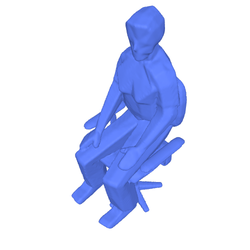
\includegraphics[width=0.13\textwidth]{Images/Unseen Category Renders/Person TARGET.png}
		\hspace{0.03\textwidth}
		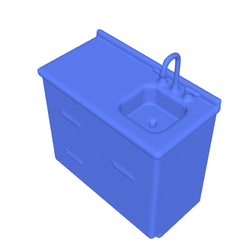
\includegraphics[width=0.13\textwidth]{Images/Unseen Category Renders/Sink TARGET.png}
		\hspace{0.03\textwidth}
		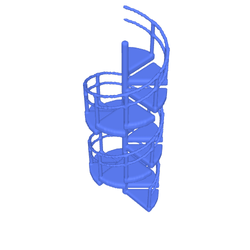
\includegraphics[width=0.13\textwidth]{Images/Unseen Category Renders/Stairs TARGET.png}
		\caption{Target ModelNet40 Shapes}
	\end{subfigure}

	\begin{subfigure}{\textwidth}
		\centering
		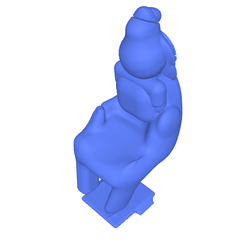
\includegraphics[width=0.13\textwidth]{Images/Unseen Category Renders/Person ShapeNet.png}
		\hspace{0.03\textwidth}
		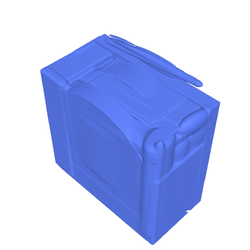
\includegraphics[width=0.13\textwidth]{Images/Unseen Category Renders/Sink ShapeNet.png}
		\hspace{0.03\textwidth}
		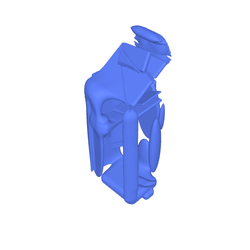
\includegraphics[width=0.13\textwidth]{Images/Unseen Category Renders/Stairs ShapeNet.png}
		\caption{ShapeNet Trained Model Reconstructions}
	\end{subfigure}
	\caption{Target shapes from the ModelNet40 dataset (top row) and reconstructions created by a model trained on the ShapeNet dataset (bottom row.)}
	\label{fig:unseen_class_renders}
\end{figure}

\begin{table}[ht]
	\centering
	\singlespace
	\footnotesize
	\setlength{\tabcolsep}{3pt}
	\setcellgapes{4pt}
	\makegapedcells
	\renewcommand{\bfdefault}{b}
	\begin{tabular}{|l|l|r|r|r|r|}
		\hline
		\makecell{Shape\\Category}& \makecell{Best\\Loss} & \makecell{Best\\CD} & \makecell{Best\\EMD} & \makecell{Best\\IoU} \\
		\Xhline{1pt}
		Person & 0.3197 & 48.27 & 848.9  & 0.4096 \\
		\hline
		Sink   & 0.2730 & 50.20 & 710.2  & 0.3725 \\
		\hline
		Stairs & 0.3344 & 84.11 & 1041.9 & 0.2437 \\
		\hline
		All    & 0.3083 & 61.76 & 868.3  & 0.3371 \\
		\hline
	\end{tabular}
	\caption{Reconstruction accuracy metrics for ModelNet40 reconstructions created by a model trained on the ShapeNet dataset.}
	\label{tab:unseen_class_comparison}
\end{table}


\section{Partial~Reconstruction~Refinement}
\label{sec:partial_recon_experiment}

A unique benefit of the cascaded refinement architecture is the ability to complete a partial reconstruction. We demonstrate this ability by creating a small subset of the ShapeNet dataset with occluded geometry. 10 mesh samples were randomly selected from each of the Airplane, Bench, Car, Chair, and Sofa categories. Since ShapeNet includes part segmentation data for each sample, we leverage this information to cleanly remove a part of each target mesh. Lastly we apply our standard SDF processing pipeline to create a 50 sample occluded shape dataset. During inference, we skip the initial prediction pass by inputting the occluded dataset sample as though it were the output from the previous cascade and runnign only two passes.

Both the single-category models and the general whole-dataset model succeed in completing the partial reconstruction. The accuracy metrics are misleading since the intact portion of the target shape skews the result positively. The reconstruction quality of the predicted missing volumes are comparable to the unseen shape category results. Volume is generally added in the correct region and not added over the existing shape, but surface detail is lacking. The single-category trained model shows signs of a learned shape template, such as the horizontal slats on the bench reconstruction that is absent from the the whole-dataset model. However, the accuracy metrics show that both perform about the same.

This experiment demonstrates that the cascades are not structured. If each cascade was designated a specific portion of a shape template to predict, the model would fail to consistently restore randomized parts of the target shape. The ability to do so indicates that the encoder can compare the target input against the initial reconstruction input to determine what volume is missing.

\newpage


\begin{figure}[ht]
	\centering
	\captionsetup[subfigure]{justification=centering}
	\begin{subfigure}{\textwidth}
		\centering
		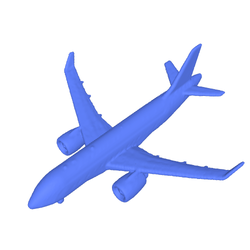
\includegraphics[width=0.1296\textwidth]{Images/Partial Reconstruction Renders/Airplane TARGET.png}
		\hspace{0.03\textwidth}
		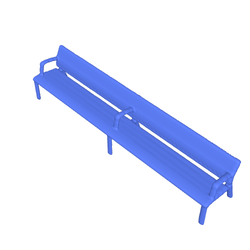
\includegraphics[width=0.1296\textwidth]{Images/Partial Reconstruction Renders/Bench TARGET.png}
		\hspace{0.03\textwidth}
		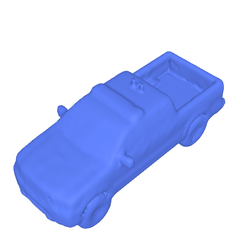
\includegraphics[width=0.1296\textwidth]{Images/Partial Reconstruction Renders/Car TARGET.png}
		\hspace{0.03\textwidth}
		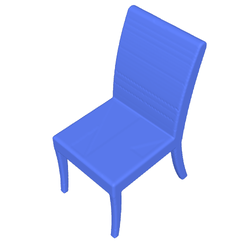
\includegraphics[width=0.1296\textwidth]{Images/Partial Reconstruction Renders/Chair TARGET.png}
		\hspace{0.03\textwidth}
		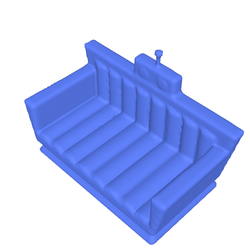
\includegraphics[width=0.1296\textwidth]{Images/Partial Reconstruction Renders/Sofa TARGET.png}
		\caption{Target}
	\end{subfigure}

	\begin{subfigure}{\textwidth}
		\centering
		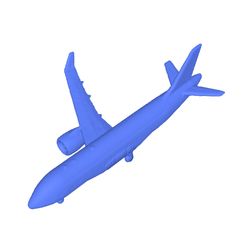
\includegraphics[width=0.1296\textwidth]{Images/Partial Reconstruction Renders/Airplane Occluded.png}
		\hspace{0.03\textwidth}
		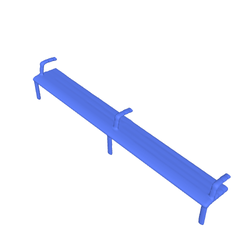
\includegraphics[width=0.1296\textwidth]{Images/Partial Reconstruction Renders/Bench Occluded.png}
		\hspace{0.03\textwidth}
		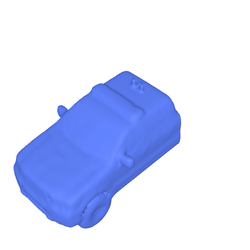
\includegraphics[width=0.1296\textwidth]{Images/Partial Reconstruction Renders/Car Occluded.png}
		\hspace{0.03\textwidth}
		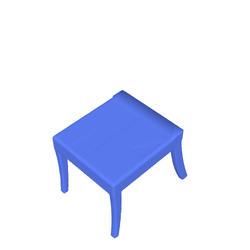
\includegraphics[width=0.1296\textwidth]{Images/Partial Reconstruction Renders/Chair Occluded.png}
		\hspace{0.03\textwidth}
		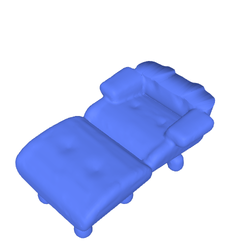
\includegraphics[width=0.1296\textwidth]{Images/Partial Reconstruction Renders/Sofa Occluded.png}
		\caption{Occluded Input}
	\end{subfigure}

	\begin{subfigure}{\textwidth}
		\centering
		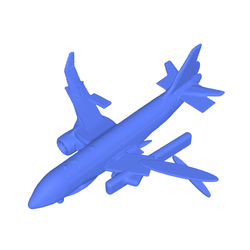
\includegraphics[width=0.1296\textwidth]{Images/Partial Reconstruction Renders/Airplane Single Category.png}
		\hspace{0.03\textwidth}
		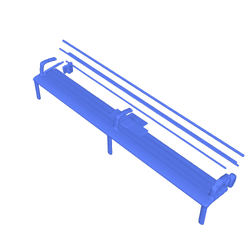
\includegraphics[width=0.1296\textwidth]{Images/Partial Reconstruction Renders/Bench Single Category.png}
		\hspace{0.03\textwidth}
		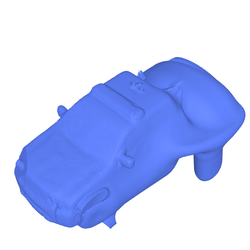
\includegraphics[width=0.1296\textwidth]{Images/Partial Reconstruction Renders/Car Single Category.png}
		\hspace{0.03\textwidth}
		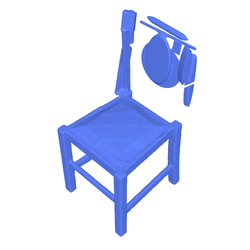
\includegraphics[width=0.1296\textwidth]{Images/Partial Reconstruction Renders/Chair Single Category.png}
		\hspace{0.03\textwidth}
		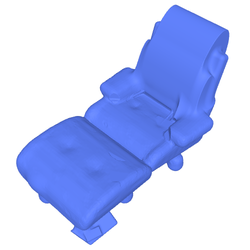
\includegraphics[width=0.1296\textwidth]{Images/Partial Reconstruction Renders/Sofa Single Category.png}
		\caption{Single-Category ShapeNet Model}
	\end{subfigure}

	\begin{subfigure}{\textwidth}
		\centering
		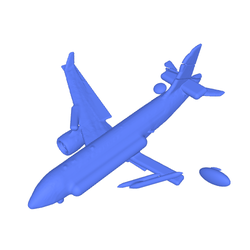
\includegraphics[width=0.1296\textwidth]{Images/Partial Reconstruction Renders/Airplane Whole Dataset.png}
		\hspace{0.03\textwidth}
		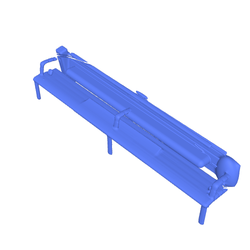
\includegraphics[width=0.1296\textwidth]{Images/Partial Reconstruction Renders/Bench Whole Dataset.png}
		\hspace{0.03\textwidth}
		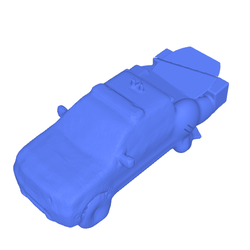
\includegraphics[width=0.1296\textwidth]{Images/Partial Reconstruction Renders/Car Whole Dataset.png}
		\hspace{0.03\textwidth}
		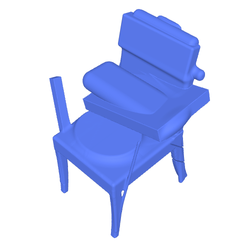
\includegraphics[width=0.1296\textwidth]{Images/Partial Reconstruction Renders/Chair Whole Dataset.png}
		\hspace{0.03\textwidth}
		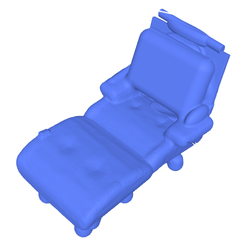
\includegraphics[width=0.1296\textwidth]{Images/Partial Reconstruction Renders/Sofa Whole Dataset.png}
		\caption{All-Category ShapeNet Model}
	\end{subfigure}
	\caption{Refinement of partially complete shapes by single and all trained ShapeNet models.}
	\label{fig:partial_recon_renders}
\end{figure}

\begin{table}[ht]
	\centering
	\singlespace
	\footnotesize
	\setlength{\tabcolsep}{3pt}
	\setcellgapes{4pt}
	\makegapedcells
	\renewcommand{\bfdefault}{b}
	\begin{tabular}{|l|l|r|r|r|}
		\hline
		\makecell{Shape Category} & \makecell{Training Set} & \makecell{Refined CD} & \makecell{Refined EMD} & \makecell{Refined IoU} \\
		\Xhline{1pt}
		\multirow{2}{*}{Airplane} & \smash[b]{Single Category} & 27.04          & 587.8          & 0.7473          \\
		                          & Whole Dataset              & \textbf{15.40} & \textbf{428.3} & \textbf{0.8146} \\
		\hline
		\multirow{2}{*}{Bench}    & \smash[b]{Single Category} & 19.52          & \textbf{463.0} & \textbf{0.7000} \\
		                          & Whole Dataset              & \textbf{12.02} & 486.4          & 0.6752          \\
		\hline
		\multirow{2}{*}{Car}      & \smash[b]{Single Category} & 33.70          & 545.4          & 0.7590          \\
		                          & Whole Dataset              & \textbf{16.88} & \textbf{490.9} & \textbf{0.7976} \\
		\hline
		\multirow{2}{*}{Chair}    & \smash[b]{Single Category} & \textbf{47.36} & \textbf{306.2} & \textbf{0.8558} \\
		                          & Whole Dataset              & 52.62          & 701.9          & 0.7109          \\
		\hline
		\multirow{2}{*}{Sofa}     & \smash[b]{Single Category} & 48.73          & 831.9          & 0.7248          \\
		                          & Whole Dataset              & \textbf{20.98} & \textbf{563.6} & \textbf{0.7724} \\
		\hline
		\multirow{2}{*}{All}      & \smash[b]{Single Category} & 35.27          & 546.9          & \textbf{0.7574} \\
		                          & Whole Dataset              & \textbf{23.58} & \textbf{534.2} & 0.7542          \\
		\hline
	\end{tabular}
	\caption{Partial shape refinement metrics for single and all category trained models.}
	\label{tab:partial_recon_comparison}
\end{table}


\section{Comparison~to~Prior~Work}
\label{sec:prior_work_comparison}

We run performance tests to compare CSG-CRN to prior works in primitive 3D reconstruction. The current state of the art models in generalized reconstruction to compare against are UCSG-Net~\cite{Kania2020}, BSP-Net~\cite{Chen2020}, and the pretrained CAPRI-Net~\cite{Yu2022} model. Works such as D\textsuperscript{2}CSG~\cite{Yu2023} and CSG-Stump~\cite{Ren2021} have better reconstruction accuracy but are not trained on multiple shape categories.

\textbf{Note:} The CSG-CRN results are for the model trained on 54 shape categories. The results will be updated once the model trained on 13 shape categories finishes.

The models are tested on a dataset of seen shape categories (ShapeNet) and unseen shape categories (ModelNet40). For the ShapeNet dataset, we selected 5 shape samples from each shape category that was in the test set of all four models being compared. For the unseen dataset, we use the same 56 shape samples in the Person, Sink, and Stairs categories that was used in the \nameref{sec:unseen_class_experiment} experiment.

The CD metrics presented in this section are not comparable to the earlier experiments. All other testing on CSG-CRN used the ChamferDistance library~\cite{Jatavallabhula2024, Ravi2020} with 10,000 samples, Marching Cubes resolution of 512, unit sphere bounds, Sum reduction and no scaling. To align with the testing methods of the previous work, the CD metrics are computed with 4,096 samples, Marching Cubes resolution of 128, box bounds, mean reduction and a final scaling of 1,000.

\begin{table}[ht]
	\centering
	\singlespace
	\footnotesize
	\setlength{\tabcolsep}{3pt}
	\setcellgapes{4pt}
	\makegapedcells
	\renewcommand{\bfdefault}{b}
	\begin{tabular}{|l|r|r|r|}
		\hline
		\makecell{Model} & \makecell{Training\\Categories} & \makecell{CD} & \makecell{IoU} \\
		\Xhline{1pt}
		CSG-CRN   & 54 & \textbf{0.600} & \textbf{0.6270} \\
		\hline
		CAPRI-Net & 13 & 0.783          & 0.5812          \\
		\hline
		BSP-Net   & 13 & 0.864          & 0.5789          \\
		\hline
		UCSG-Net  & 13 & 2.758          & 0.5303          \\
		\hline
	\end{tabular}
	\caption{Comparison of models on ShapeNet dataset.}
	\label{tab:prior_work_seen_comparison}
\end{table}

\begin{table}[ht]
	\centering
	\singlespace
	\footnotesize
	\setlength{\tabcolsep}{3pt}
	\setcellgapes{4pt}
	\makegapedcells
	\renewcommand{\bfdefault}{b}
	\begin{tabular}{|l|r|r|r|r|r|r|r|r|}
		\hline
		\multicolumn{1}{|c|}{\multirowcell{2}{Model}} & \multicolumn{2}{c|}{Person} & \multicolumn{2}{c|}{Sink} & \multicolumn{2}{c|}{Stairs} & \multicolumn{2}{c|}{All} \\
		\cline{2-9}
		                       & \makecell{CD} & \makecell{IoU} & \makecell{CD} & \makecell{IoU} & \makecell{CD} & \makecell{IoU} & \makecell{CD} & \makecell{IoU} \\
		\Xhline{1pt}
		CSG-CRN   & \textbf{1.050} & \textbf{0.4177} & \textbf{1.224} & \textbf{0.3702} & \textbf{1.961} & \textbf{0.2445} & \textbf{1.437} & \textbf{0.3389} \\
		\hline
		CAPRI-Net & 1.967          & 0.3670          & 1.638          & 0.3316          & 4.304          & 0.2250          & 2.684          & 0.3036          \\
		\hline
		BSP-Net   & 2.823          & 0.2940          & 2.805          & 0.2577          & 5.325          & 0.1812          & 3.710          & 0.2407          \\
		\hline
		UCSG-Net  & 3.162          & 0.2856          & 3.315          & 0.2568          & 8.458          & 0.1728          & 5.108          & 0.2351          \\
		\hline
	\end{tabular}
	\caption{Comparison of models on ModelNet40 dataset.}
	\label{tab:prior_work_unseen_comparison}
\end{table}

\begin{table}[ht]
	\centering
	\singlespace
	\footnotesize
	\setlength{\tabcolsep}{3pt}
	\setcellgapes{4pt}
	\makegapedcells
	\renewcommand{\bfdefault}{b}
	\begin{tabular}{|l|r|r|r|r|r|r|r|r|r|r|r|r|}
		\hline
		\multicolumn{1}{|c|}{\multirowcell{2}{Model}} & \multicolumn{2}{c|}{Airplane} & \multicolumn{2}{c|}{Bench} & \multicolumn{2}{c|}{Car} & \multicolumn{2}{c|}{Chair} & \multicolumn{2}{c|}{Sofa} & \multicolumn{2}{c|}{All} \\
		\cline{2-13}
		                       & \makecell{CD} & \makecell{IoU} & \makecell{CD} & \makecell{IoU} & \makecell{CD} & \makecell{IoU} & \makecell{CD} & \makecell{IoU} & \makecell{CD} & \makecell{IoU} & \makecell{CD} & \makecell{IoU} \\
		\Xhline{1pt}
		CSG-CRN   & \textbf{0.163} & \textbf{0.6817} & \textbf{0.614} & \textbf{0.5149} & \textbf{0.515} & \textbf{0.6642} & \textbf{0.478} & \textbf{0.6660} & \textbf{0.514} & \textbf{0.7797} & \textbf{0.446} & \textbf{0.6715} \\
		\hline
		CSG-Stump & 0.500 & 0.4465 & 0.994 & 0.4666 & 0.626 & 0.6503 & 1.205 & 0.5217 & 0.758 & 0.7474 & 0.804 & 0.5734 \\
		\hline
	\end{tabular}
	\caption{}
	\label{tab:prior_work_single_category_comparison}
\end{table}


\section{Photogrammetry~Reconstruction}
\label{sec:photogrammetry_reconstruction}

A unique benefit of the point cloud input format for CSG-CRN is the flexibility in acquiring input data. Surface point clouds can be easily generated using photogrammetry techniques. And a surface point cloud can be augment into an SDF point cloud input suitable for CSG-CRN.

To demonstrate, we took videos circling 360 degrees around three objects. An open source tool COLMAP~\cite{schoenberger2016sfm} was used to extract frames, create depths maps, and output a point cloud scan. Some pre-processing is applied to the raw points to remove outliers, orient the shape into a canonical frame, and remove the floor plane. Similar to the ShapeNet dataset processing, near-surface sample points can be generated by applying Gaussian noise to the surface points. Distances for both near-surface and uniform points can be approximated using a K-d tree to find the closest surface sample.

We apply this process to produce three SDF shape samples to run inference on. We experiment with the single-category model trained on the ShapeNet Car subset and the all-categories model. The car subject is a known shape category that both models trained on while the rabbit and teddy bear subjects are unknown categories. Since there is no ground-truth mesh to validate against, we compute accuracy as the IoU metric between the reconstruction and input SDF point clouds.

As expected, the single-category model produced the best reconstruction of the four. It produces a smooth surface and a more defined windshield than the all-categories model does. Both models were able to reconstruct the windows missing from the photogrammetry scan due to glare. The all-category model produced a decent approximation of the rabbit. The general shape and contains a head and ears, but it lacks much detail. The reconstruction of the teddy bear sample is the worst result with the model failing to reconstruct the arms and legs.


\begin{figure}[ht]
	\centering
	\captionsetup[subfigure]{justification=centering}
	\begin{subfigure}{\textwidth}
		\centering
		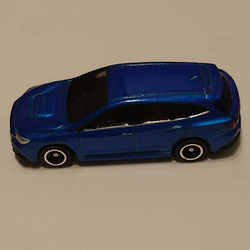
\includegraphics[width=0.13\textwidth]{Images/Photogrammetry Renders/Car Video Frame.png}
		\hspace{0.03\textwidth}
		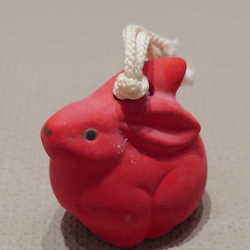
\includegraphics[width=0.13\textwidth]{Images/Photogrammetry Renders/Rabbit Bell Video Frame.png}
		\hspace{0.03\textwidth}
		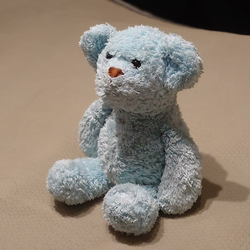
\includegraphics[width=0.13\textwidth]{Images/Photogrammetry Renders/Teddy Bear Video Frame.png}
		\caption{Video Scan}
	\end{subfigure}

	\begin{subfigure}{\textwidth}
		\centering
		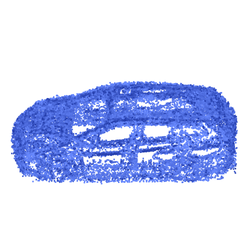
\includegraphics[width=0.13\textwidth]{Images/Photogrammetry Renders/Car Point Cloud.png}
		\hspace{0.03\textwidth}
		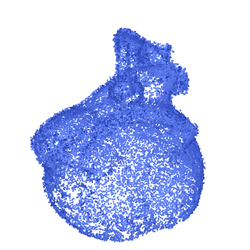
\includegraphics[width=0.13\textwidth]{Images/Photogrammetry Renders/Rabbit Bell Point Cloud.png}
		\hspace{0.03\textwidth}
		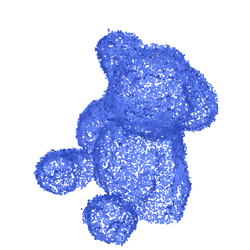
\includegraphics[width=0.13\textwidth]{Images/Photogrammetry Renders/Teddy Bear Point Cloud.png}
		\caption{Extracted Point Cloud}
	\end{subfigure}

	\begin{subfigure}{\textwidth}
		\centering
		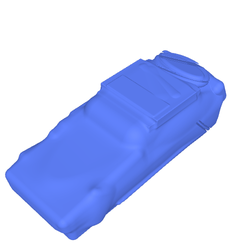
\includegraphics[width=0.13\textwidth]{Images/Photogrammetry Renders/Car Reconstruction Whole Dataset.png}
		\hspace{0.03\textwidth}
		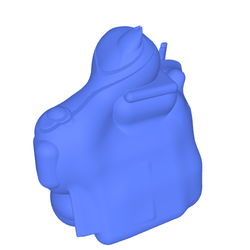
\includegraphics[width=0.13\textwidth]{Images/Photogrammetry Renders/Rabbit Bell Reconstruction.png}
		\hspace{0.03\textwidth}
		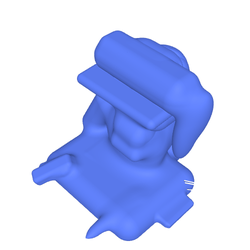
\includegraphics[width=0.13\textwidth]{Images/Photogrammetry Renders/Teddy Bear Reconstruction.png}

		\footnotesize
		\makebox[0.13\textwidth]{IoU 0.8865}
		\hspace{0.03\textwidth}
		\makebox[0.13\textwidth]{IoU 0.7252}
		\hspace{0.03\textwidth}
		\makebox[0.13\textwidth]{IoU 0.6242}
		\caption{All-Category ShapeNet Model Reconstruction}
	\end{subfigure}

	\begin{subfigure}{\textwidth}
		\centering
		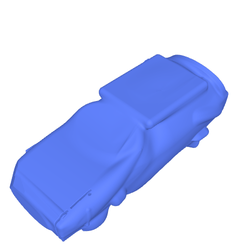
\includegraphics[width=0.13\textwidth]{Images/Photogrammetry Renders/Car Reconstruction Single Category.png}

		\footnotesize
		\makebox[0.13\textwidth]{IoU 0.8986}
		\caption{Single-Category Car Model Reconstruction}
	\end{subfigure}
	\caption{Reconstructing CSG Models from scans of real-world objects. The first row depicts frames from the video scan. The second row shows the surface point clouds extracted through photogrammetry. And the last two rows show CSG-CRN reconstructions.}
	\label{fig:photogrammetry_renders}
\end{figure}



